\documentclass[12pt, a4paper]{article}

\usepackage{amsmath, amssymb, titling}
\usepackage[margin=2.5cm]{geometry}
\usepackage[colorlinks=true, linkcolor=black, urlcolor=black, citecolor=black]{hyperref}
\usepackage{graphicx}
\usepackage{caption}
\usepackage{subcaption}
\usepackage{float}
\usepackage{fancyhdr, lastpage}
\usepackage{fourier-orns}
\usepackage{xcolor}
\usepackage{matlab-prettifier}
\usepackage[T1]{fontenc}

\renewcommand\maketitlehooka{\null\mbox{}\vfill}
\renewcommand\maketitlehookd{\vfill\null}
\renewcommand{\headrule}{
\vspace{-5pt}\hrulefill
\raisebox{-2.1pt}{\quad\leafleft\decoone\leafright\quad}\hrulefill}

\title{Satellite Orbit Control \\ HW9}
\author{Almog Dobrescu\\\\ID 214254252}

\pagestyle{fancy}
\cfoot{Page \thepage\ of \pageref{LastPage}}

\begin{document}

\maketitle

\thispagestyle{empty}
\newpage
\setcounter{page}{1}

\tableofcontents
\vfil
\listoffigures
\newpage

\section{Given}
A communication satellite is placed in a geostationary orbit above longitude $30^\circ\mathrm{E}$.
\begin{equation}
    \begin{matrix}
        T=8.6164\cdot10^4\left[\mathrm{sec}\right]\rightarrow a=4.2164\cdot10^4\left[\mathrm{km}\right] && \lambda_n=30^\circ && e=0 && i=0 \\
    \end{matrix}
\end{equation}
The longitude tolerance is $\Delta\lambda=\pm0.05^\circ$

\subsection{Desired}

\subsection{Limitations}
The thrust is only at the $\pm y$ direction and:
\begin{equation}
    a_{\mathrm{max}}=1\cdot10^{-7}\left[\frac{\mathrm{km}}{\mathrm{sec}^2}\right]
\end{equation}

\section{Control}
\subsection{East-West Control}
\subsubsection{Drift Duo to Tesseral Harmonics}
The gravity component normal to the radius changes the orbit period so the satellite moves toward the closest equilibrium point. The force component creates a tangential acceleration, which is equivalent to the angular acceleration of the longitude line underneath the satellite:
\begin{equation}
    a\ddot{\lambda}=\vec{f}\cdot\vec{v}
\end{equation}
The change in the semi-major axis and the longitude line over one cycle:
\begin{equation}
    \begin{array}{rcl}
        \displaystyle\frac{da}{dt}&=&\displaystyle-12anJ_{22}\left(\frac{Re}{a}\right)^2\sin\left(2\left(\lambda-\lambda_{22}\right)\right) \\\\
        \displaystyle\frac{d^2\lambda}{dt^2}&=&\displaystyle-\frac{3}{2}\frac{n}{a}\frac{da}{dt}
    \end{array}
\end{equation}
Where:
\begin{equation}
    \begin{array}{rcl}
        \displaystyle J_{22}&=&\displaystyle\left(C_{22}^2+S_{22}^2\right)^{\frac{1}{2}} \\\\
        \displaystyle\lambda_{22}&=&\displaystyle\tan^{-1}\left(\frac{S_{22}}{C_{22}}\right)=-14.9^\circ
    \end{array}
\end{equation}
After substitution:
\begin{equation}
    \begin{matrix}
        \begin{array}{rcl}
            \dot{a}&=&\displaystyle0.132\sin\left(2\left(\lambda-\lambda_s\right)\right)\left[\frac{\mathrm{km}}{\mathrm{day}}\right] \\\\
            \ddot{\lambda}&=&\displaystyle-0.00168\sin\left(2\left(\lambda-\lambda_s\right)\right)\left[\frac{\mathrm{deg}}{\mathrm{day}^2}\right]
        \end{array} && \substack{\displaystyle\lambda_s\text{ is the closest stable}\\\\\displaystyle\text{equilibrium point }75^\circ\ \mathrm{or}\ 255^\circ}
    \end{matrix}
\end{equation}
Since the tolerance is small:
\begin{equation}
    \begin{array}{c}
        \ddot{\lambda}=-K\sin\left(2\left(\lambda_n-\lambda_s\right)\right)=\ddot{\lambda}_n \\\\
        \lambda=\displaystyle\frac{1}{2\ddot{\lambda}_n}\left(\dot{\lambda}-\dot{\lambda}_0\right)^2+\frac{\dot{\lambda}_0}{\ddot{\lambda}_n}+\lambda_0
    \end{array}
\end{equation}
The initial conditions of the satellite:
\begin{equation}
    \begin{matrix}
        \lambda_0=\lambda_n-\Delta\lambda && \dot{\lambda}_0=-2\mathrm{\ sgn}\left(\ddot{\lambda}_n\right)\sqrt{-\ddot{\lambda}_n\Delta\lambda}
    \end{matrix}
\end{equation}
The velocit pulse needes to change $-\dot{\lambda}_0$ into $\dot{\lambda}_0$:
\begin{equation}
    \Delta n=2\dot{\lambda}_0
\end{equation}
The relation between the change in angular velocit and the semi-major axis:
\begin{equation}
    \begin{array}{c}
        \displaystyle n^2=\frac{\mu}{a^3}\rightarrow\frac{\Delta a}{a}=-\frac{2}{3}\frac{\Delta n}{n} \\
        \Downarrow \\
        \displaystyle \Delta v=\left|\frac{\mu}{2a^2v}\Delta a\right|=\frac{a}{3}\left|\Delta n\right|=\frac{2a}{3}\left|\dot{\lambda}_0\right|
    \end{array}
\end{equation}
and the friquency of pulses:
\begin{equation}
    t_m=2\left|\frac{\dot{\lambda}_0}{\ddot{\lambda}_n}\right|
\end{equation}
The change in altitude between to corections:
\begin{equation}
    \Delta a=0.132\sin\left(2\left(\lambda-\lambda_s\right)\right)t_m\left[\mathrm{km}\right]
\end{equation}

% \subsection{Drift due to The Tesseral Harmonics}
% \begin{equation}
%     \begin{array}{l}
%         \displaystyle\frac{da}{dt}=6.06\sin\left(2\left(\lambda-27.8^\circ\mathrm{E}\right)\right)-1.48\sin\left(4\left(\lambda-30.28^\circ\mathrm{E}\right)\right)+0.19\sin\left(2\left(\lambda-31.92^\circ\mathrm{E}\right)\right)\left[\frac{\mathrm{m}}{\mathrm{day}}\right] \\\\
%         \displaystyle\frac{d^2\lambda}{dt^2}=\frac{3n}{4a}\frac{da}{dt}
%     \end{array}
% \end{equation}

\newpage

\section{The Results}
\subsection{Part A}
\begin{equation}
    \begin{matrix}
        \begin{array}{rcl}
            \ddot{\lambda}_n&=&\displaystyle-0.00168\sin\left(2\left(30^\circ-75^\circ\right)\right)=0.0017\left[\frac{\mathrm{deg}}{\mathrm{day}^2}\right] \\\\
            \dot{\lambda}_0&=&\displaystyle-2\mathrm{\ sgn}\left(\ddot{\lambda}_n\right)\sqrt{-\ddot{\lambda}_n\Delta\lambda}=-0.0183\left[\frac{\mathrm{deg}}{\mathrm{day}}\right] \\
        \end{array} \\
        \Downarrow \\
        \colorbox{yellow}{$\displaystyle t_m=2\left|\frac{\dot{\lambda}_0}{\ddot{\lambda}_n}\right|=2\left|\frac{-0.0183}{0.0017}\right|=21.8218\left[\mathrm{day}\right]$} \\
        \Downarrow \\
        \colorbox{yellow}{$\displaystyle\Delta a=0.132\sin\left(2\left(30^\circ-75^\circ\right)\right)t_m=-2.8805\left[\mathrm{km}\right]$}
    \end{matrix}
\end{equation}

\subsection{Part C}
In order to test the worst scenario, the initial condition for the rate of change of the longitude line will be its maximal value:
\begin{equation}
    \dot{\lambda}_0=\pm0.0183\left[\frac{\mathrm{deg}}{\mathrm{day}}\right]
\end{equation}
and the initial longitude line will be the nominal one:
\begin{equation}
    \lambda_0=\lambda_n=30^\circ
\end{equation}
By assuming that the amplitude of the change of the semi-major axis is constant we get the range of longitudes:
\begin{figure}[H]
    \centering
    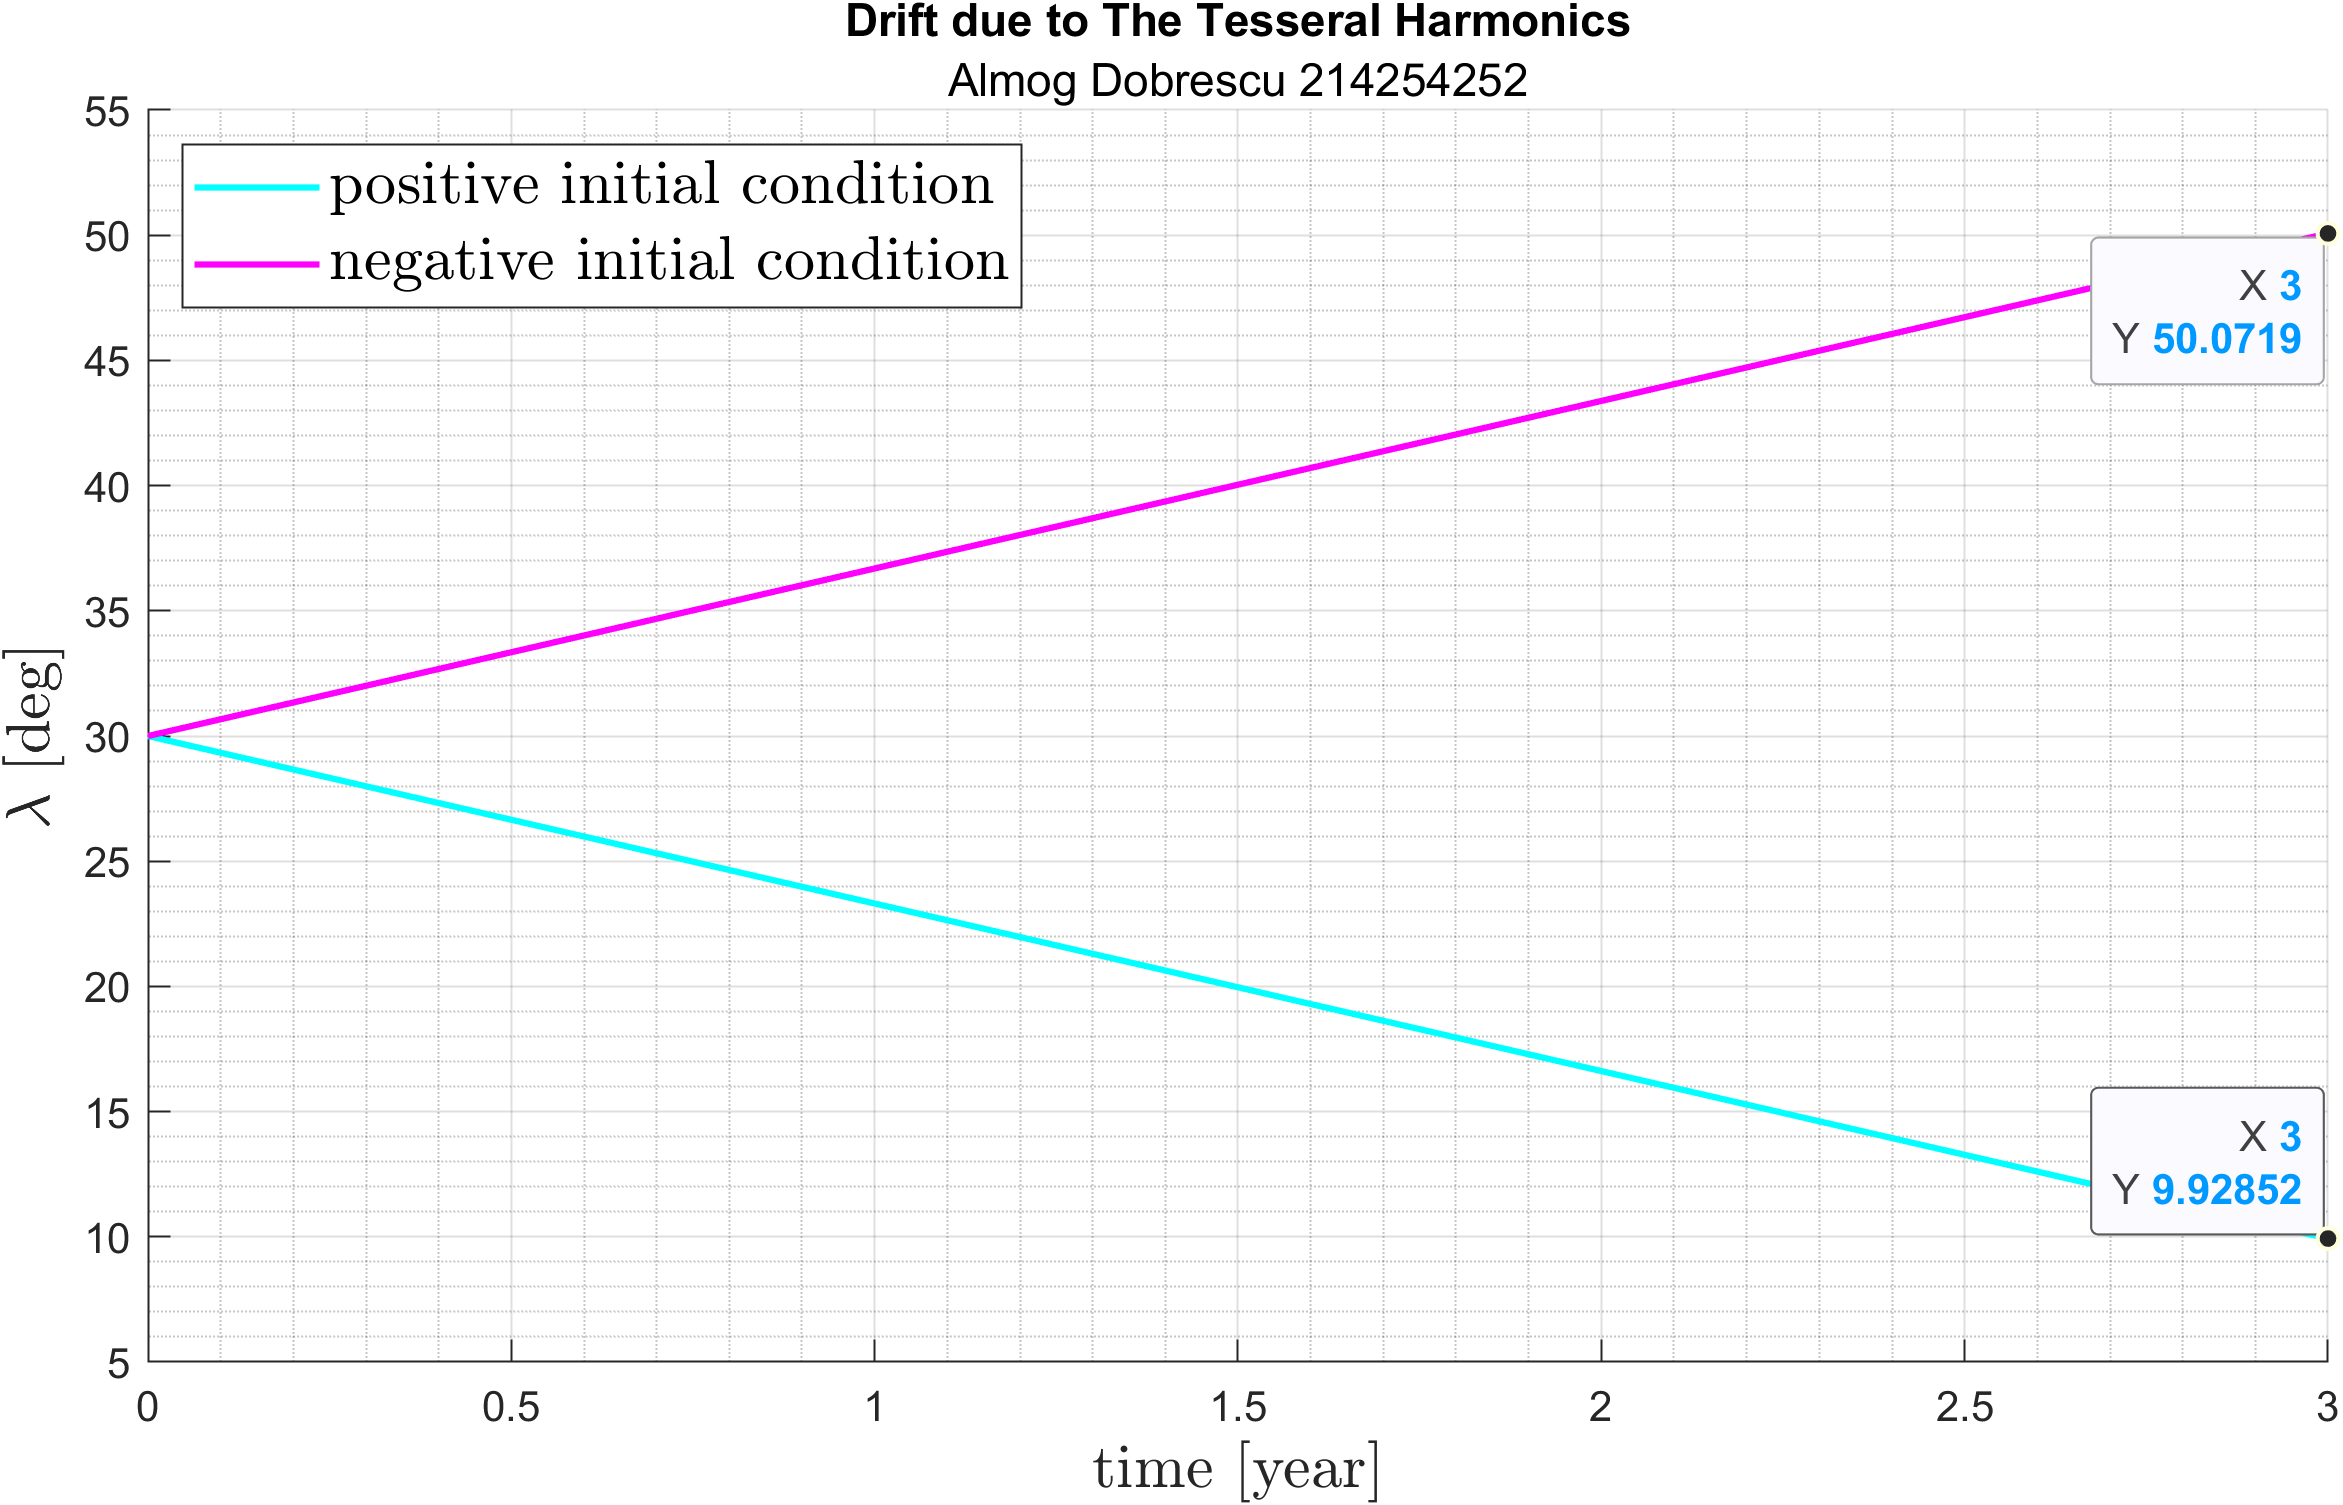
\includegraphics[width=0.7\textwidth]{images/graph1.png}
    \caption{Longitude vs. Time}
    \label{fig:longitude_vs_time}
\end{figure}
We can see that the maximal longitude range is $\colorbox{yellow}{$\pm20.0719^\circ$}$.

\newpage

\appendix
\section{The Code}
\begin{lstinputlisting}[captionpos=b,stringstyle=\color{magenta},frame=single, numbers=left, style=MatLab-editor, basicstyle=\mlttfamily\small, caption={The code},mlshowsectionrules=true]{./matlab/SOC_hw9.m}
\end{lstinputlisting}

\end{document}